\section{Componenti di reti sequenziali}
Le componenti standard implementate sotto forma di rete sequenziale sono di fatto registri e
memorie. In particolare andremo a parlare di
\begin{itemize}
	\item Registri e banchi di registri.
	\item Memorie: statiche, dinamiche e ROM.
\end{itemize}
Dei registri da 1 bit abbiamo già parlato in precedenza, proseguiamo con le altre componenti anche
se riprenderemo il discorso sulle memorie più avanti in modo più approfondito.

\subsection{Banco di registri}
I banchi di registri sono una prima forma di \textbf{memoria} in grado di memorizzare più
\emph{parole} le quali sono accessibili tramite un \textbf{indirizzo}. Di seguito un banco da 2
registri.
\begin{center}
	\begin{tikzpicture}
		\draw[->, >=Stealth] (0, 0) node[label=left:EN] {} -- (1, 0); % EN
		\draw[thick] (1, -0.5) -- (1, 0.5) -- (1.5, 0.75) -- (1.5, -0.75) -- cycle; % DEMUX
		\draw[thick] (2.5, 0.75) rectangle (3.5, 0.25); % R1
		\draw[thick] (2.5, -0.75) rectangle (3.5, -0.25); % R2
		\draw[thick] (4.5, -0.75) -- (4.5, 0.75) -- (5, 0.5) -- (5, -0.5) -- cycle; % MUX
		\draw[->, >=Stealth] (5, 0) -- (6, 0) node[label=right:out] {}; % OUT
		\draw[->, >=Stealth] (1.5, 0.375) -- (2.5, 0.375); % demux -> R1
		\draw[->, >=Stealth] (1.5, -0.625) -- (2.5, -0.625); % demux -> R2

		% clock
		\draw[->, >=Stealth, dashed] (1.875, 0.625) -- (2.5, 0.625);
		\draw[->, >=Stealth, dashed] (1.875, -0.375) -- (2.5, -0.375);
		\draw[dashed] (1.875, 1.5) node[label=above:clock] {} -- (1.875, -0.375);

		\draw[->, >=Stealth] (3.5, 0.5) -- (4.5, 0.5); % R1 -> MUX
		\draw[->, >=Stealth] (3.5, -0.5) -- (4.5, -0.5); % R2 -> MUX

		% INPUT
		\draw[->, >=Stealth] (3, 1.5) node[label=above:IN] {} -- (3, 0.75);
		\draw[->, >=Stealth] (3, 1.125) to[short, *-] (4, 1.125) -- (4, 0) -- (3, 0) -- (3, -0.25);

		% INDIRIZZAMENTO
		\draw[->, >=Stealth] (0, -1.25) node[label=left:IND] {} to[short, -*] (1.25, -1.25) --
		(1.25, -0.625);
		\draw[->, >=Stealth] (1.25, -1.25) -- (4.75, -1.25) -- (4.75, -0.625);
	\end{tikzpicture}
\end{center}
Come possiamo vedere, tramite il segnale di IND riusciamo a scrivere IN su uno specifico registro
scelto dal demultiplexer, lo stesso IND viene inviato al multiplexer alla fine per riuscire a
leggere la locazione di memoria indirizzata.

Questo metodo fa uso di registri così come li abbiamo definiti in precedenza e consuma un numero di
transistor molto alto.

\subsection{Memorie dinamiche}
Le \textbf{memorie dinamiche} sono implementate in modo tale da permetterci di risparmiare più
transistor ma hanno il continuo bisogno di \emph{"rinfrescare"} il loro contenuto per evitare che
questo vada perso.

Similmente ai banchi di memoria, abbiamo un demultiplexer a cui diamo in ingresso una parola da
scrivere e l'indirizzo a cui scriverla. L'output del demultiplexer è collegato ad una griglia
con un numero di righe pari al numero massimo di parole memorizzabili nella memoria e un numero
di colonne pari alla lunghezza in bit di ognuna delle parole.
\begin{center}
	\begin{tikzpicture}
		\draw[thick] (1, -0.5) -- (1, 0.5) -- (1.5, 0.75) -- (1.5, -0.75) -- cycle; % DEMUX

		% GRID
		\foreach \i in {-0.5, -0.25, 0, 0.25, 0.5}
		\draw[thick] (1.5, \i) -- (3, \i);

		\foreach \i in {1.75, 2, 2.25, 2.5, 2.75}
		\draw[thick] (\i, 0.75) -- (\i, -0.75);

		\draw[->, >=Stealth] (0, 0) node[label=left:IN] {} -- (1, 0);
		\draw[->, >=Stealth] (0, -1) node[label=left:IND] {} -- (1.25, -1) -- (1.25, -0.625);
		\draw[->, >=Stealth] (2.25, -1) -- (2.25, -1.875) node[label=right:OUT] {};
	\end{tikzpicture}
\end{center}
Se volessimo vedere più da vicino la griglia, nello specifico i punti di incrocio, saremmo in grado
di osservare che è presente un transistor il quale si comporta come un condensatore (mantiene una
carica elettrica) e come un interruttore poiché, quando è chiuso, mette in collegamento la riga con
la colonna, viceversa, quando è aperto non c'è alcun contatto.
\begin{center}
	\begin{tikzpicture}
		\draw[thick] (0, 0) -- (1.5, 0);
		\draw[thick] (1.25, 0.25) -- (1.25, -1.25);
		\draw[thick, red] (0.75, 0) -- (1.25, -0.5);
		\draw[->, >=Stealth] (0, -1) node[label=left:transistor] {} -- (0.875, -0.375);
	\end{tikzpicture}
\end{center}
Le linee orizzontali e verticali non si toccano a meno che il transistor non sia chiuso. Quando
facciamo passare un segnale 1 su una certa riga, questo incontra tutti i transistor, per tutti
quelli trovati chiusi, l'1 viene trasmesso sulla rispettiva colonna e inviato in output. Per ogni
transistor aperto, l'1 non si propagherà e dunque avremmo uno 0 in output. In questo modo è
possibile \textbf{leggere} la parola all'indirizzo IND.

Se invece volessimo \textbf{scrivere} una parola all'indirizzo IND dovremmo manipolare i bit sulle
colonne in modo tale che formino la parola desiderata. Come prima inviamo un segnale 1 all'indirizzo
scelto e i transistor chiusi tratterrano una carica elettrica in grado di memorizzare tutti gli 1
della parola. Sui bit messi a 0 i transistor avranno una configurazione aperta e quindi daranno in
output uno 0.

\subsection{Memorie statiche}
Le memorie statiche hanno una struttura a griglia come quelle dinamiche ma hanno una struttura più
complessa per quanto riguarda il collegamento tra righe e colonne. Si usano infatti due porte
\verb|NOT| e due transistor (T1 e T2) per la lettura e la scrittura dei bit. Come conseguenze
abbiamo un maggior consumo di spazio sul silicio ma anche una maggiore velocità nell'accesso alla
memoria.
\begin{center}
	\begin{circuitikz}
		\node[not port] (not1) at (0, 1) {};
		\node[not port, rotate=180] (not2) at (0, -1) {};

		\draw (-2, 0) node[label=left:T1] {} -- (-1, 0) -- (-1, 1) -- (not1.in);
		\draw (not1.out) -- (1, 1) -- (1, 0);
		\draw (2, 0) node[label=right:T2] {} -- (1, 0) -- (1, -1) -- (not2.in);
		\draw (not2.out) -- (-1, -1) -- (-1, 0);
	\end{circuitikz}
\end{center}
Inotre non è più necessario \emph{rinfrescare} il contenuto della memoria in continuazione poiché
questo tipo di memoria è in grado di trattenere l'informazione in modo autonomo.

\subsubsection{ROM}
Le \textbf{ROM} (Read Only Memory) sono molto simili, come struttura, alle RAM viste fino ad ora
ma non abbiamo alcun meccanismo di controllo sui transistor che collegano le righe alle colonne
della griglia. Abbiamo un collegamento diretto (nel caso volessimo trasmettere un 1) oppure
l'assenza di quest'ultimo (nel caso volessimo trasmettere uno 0).

\subsubsection{Considerazioni sulle RAM}
Queste appena descritte sono dette memorie \textbf{RAM} (Random Access Memory) poiché non è
necessario leggere tutte le locazioni in sequenza ma possiamo accedere direttamente alla locazione
desiderate. Comparando i tre tipi di RAM che abbiamo visto fino ad ora possiamo dire che
\begin{itemize}
	\item I registri sono i più veloci per quanto riguarda lettura e scrittura ma sono quelli
	      occupano più spazio sul silicio a parità di capienza.
	\item Le memorie dinamiche sono quelle più lente ma che occupano meno spazio sul silicio.
	\item Le memorie statiche si collocano a metà tra queste due per quanto riguarda velocità e
	      spazio occupato.
\end{itemize}
A seconda dell'uso che se ne fa e dei contesti sarà necessario scegliere un tipo di RAM piuttosto
che l'altro.

\subsection{Memorie modulari}\label{ss: modulari}
Da questo momento considereremo i registri come una sorta di vettore di registri, il quale prende
ad esempio in input tre indirizzi e ha 2 uscite. Questo perché se, come vedremo più avanti, in
assembler volessimo eseguire un'operazione di \verb|ADD| tra un registro \verb|R2| e un registro
\verb|R3| e volessimo salvare il risultato in un registro \verb|R1|, questo schema ci sarà molto
utile
\begin{center}
	\begin{tikzpicture}
		\draw[thick] (-0.75, -0.75) rectangle (0.75, 0.75);
		\node at (0, 0) {REG};
		\draw[->, >=Stealth] (-1.75, 0.5) node[label=left:\scriptsize{IND1}]	{} -- (-0.75, 0.5);
		\draw[->, >=Stealth] (-1.75, 0) node[label=left:\scriptsize{IND2}] {} -- (-0.75, 0);
		\draw[->, >=Stealth] (-1.75, -0.5) node[label=left:\scriptsize{IND3}]{} -- (-0.75, -0.5);

		\draw[->, >=Stealth] (-1.5, 1) node[label=left:\scriptsize{IN}] {} -- (0, 1) -- (0, 0.75);

		\draw[->, >=Stealth] (0.75, 0.25) -- (1.75, 0.25) node[label=right:\scriptsize{OUT1}] {};
		\draw[->, >=Stealth] (0.75, -0.25) -- (1.75, -0.25) node[label=right:\scriptsize{OUT2}] {};
	\end{tikzpicture}
\end{center}
Possiamo quindi leggere o scrivere più indirizzi di memoria in un singolo ciclo di clock. Per le
RAM invece dobbiamo, in generale, eseguire più cicli di clock. Possiamo anche vedere le memorie
come moduli di parole da $n$ bit, concatenabili e a cui è possibile inviare in uno stesso ciclo di
clock lo stesso indirizzo e il segnale di \verb|ENABLE|. In questo modo otteniamo una parola che
è più lunga del singolo modulo.

Se ad esempio avessimo a disposizione moduli da 1M parole di 32 bit e volessimo una memoria da 2M
parole, sarebbe possibile concatenare due di questi moduli.

Prima di tutto consideriamo che per indirizzare 1M servono $\log_2 (1 \times 10^6) = 20$ bit,
quindi per indirizzarne 2 servono 21 bit. Avremmo quindi 1 bit che sceglie quale dei due moduli
andare a leggere o scrivere e i restanti bit che andranno ad accedere la locazione di memoria
corretta.
\begin{center}
	\begin{tikzpicture}
		\draw[thick] (-2, 0) rectangle (-0.5, 1.5);
		\draw[thick] (0.5, 0) rectangle (2, 1.5);

		\draw[thick] (-1, -1) -- (1, -1) -- (0.75, -1.5) -- (-0.75, -1.5) -- cycle;
		\draw[thick] (-1, 2) rectangle (1, 2.25)
		(-0.75, 2.25) -- (-0.75, 2);

		\draw[->, >=Stealth] (-1, 2.125) -- (-2.5, 2.125) -- (-2.5, -1.25) -- (-0.875, -1.25);
		\draw[->, >=Stealth] (-1.25, 0) -- (-1.25, -0.5) -- (-0.5, -0.5) -- (-0.5, -1);
		\draw[->, >=Stealth] (1.25, 0) -- (1.25, -0.5) -- (0.5, -0.5) -- (0.5, -1);
		\draw[->, >=Stealth] (0, 2) to[short, -*] (0, 0.75) -- (-0.5, 0.75);
		\draw[->, >=Stealth] (0, 0.75) -- (0.5, 0.75);
		\draw[->, >=Stealth] (0, -1.5) -- (0, -2);

		\node at (-1.75, 1.25) {0};
		\node at (0.75, 1.25) {1};
	\end{tikzpicture}
\end{center}
Se il bit che determina quale modulo andare a leggere o scrivere è il più significativo parleremo
di memoria modulare \textbf{sequenziale}, il cui schema logico è il seguente
\begin{center}
	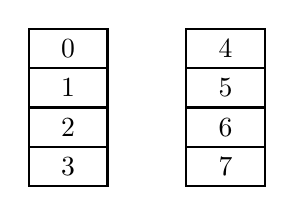
\begin{tikzpicture}
		\draw[thick] (0, 0) rectangle (1, 2);
		\draw[thick] (2, 0) rectangle (3, 2);

		\foreach \i in {1.5, 1, 0.5}{
				\draw[thick] (0, \i) -- (1, \i);
				\draw[thick] (2, \i) -- (3, \i);
			}

		\node at (0.5, 1.75) {0};
		\node at (0.5, 1.25) {1};
		\node at (0.5, 0.75) {2};
		\node at (0.5, 0.25) {3};

		\node at (2.5, 1.75) {4};
		\node at (2.5, 1.25) {5};
		\node at (2.5, 0.75) {6};
		\node at (2.5, 0.25) {7};
	\end{tikzpicture}
\end{center}
Se invece il bit in questione fosse il meno significativo dell'indirizzo quella che otteniamo è una
memoria modulare \textbf{interlacciata}, il cui schema logico è il seguente
\begin{center}
	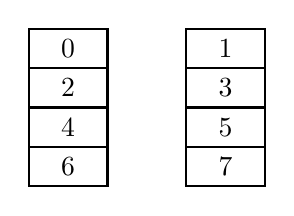
\begin{tikzpicture}
		\draw[thick] (0, 0) rectangle (1, 2);
		\draw[thick] (2, 0) rectangle (3, 2);

		\foreach \i in {1.5, 1, 0.5}{
				\draw[thick] (0, \i) -- (1, \i);
				\draw[thick] (2, \i) -- (3, \i);
			}

		\node at (0.5, 1.75) {0};
		\node at (0.5, 1.25) {2};
		\node at (0.5, 0.75) {4};
		\node at (0.5, 0.25) {6};

		\node at (2.5, 1.75) {1};
		\node at (2.5, 1.25) {3};
		\node at (2.5, 0.75) {5};
		\node at (2.5, 0.25) {7};
	\end{tikzpicture}
\end{center}
Come possiamo vedere, in questo caso abbiamo che le locazioni di memoria sono enumerate saltando
costantemente da un modulo all'altro. Questo significa che se avessimo bisogno di scrivere in
memoria una parola da 64 bit potremmo farlo andando a scrivere prima nella locazione $m_i$ e poi in
quella $m_{i+1}$ che si troverà sull'altro modulo ma allo stesso livello.

Se adessimo eliminassimo il multiplexer alla fine del circuito mostrato in precedenza otterremmo
due uscite da 32 bit, ognuna con metà della parola da 64 bit. \`E quindi possibile leggere due
parole in un singolo ciclo di clock in questo modo.

Con il modello sequenziale avremmo avuto bisogno di due cicli di clock in quanto la locazione
$m_{i+1}$ si sarebbe trovata all'interno dello stesso modulo.

\subsection{Da rete combinatoria a sequenziale}
Ogni rete combinatoria si può implementare tramite una memoria. In generale, se abbiamo una rete
combinatoria con un certo numero di ingressi e un certo numero di uscite, sarà possibile salvare
ognuna delle possibili usciti in memoria utilizzando come indirizzo gli ingressi che generano tali
uscite.

Implementare tutte le componenti in questo modo è ovviamente svantaggioso. Il vantaggio si ha se
teniamo di conto che la memoria può essere riscritta e quindi, a patto di rispettare il numero di
bit in ingresso, in uscita e quelli memorizzabili sulla memoria sarebbe possibile implementare più
moduli su una singola memoria, riscrivendola quando necessario. Per riuscire nell'intento possiamo
\begin{enumerate}
	\item Derivare l'automa.
	\item Derivare la funzione che calcola le uscite.
	\item Derivare la funzione che calcola lo stato successivo.
	\item Implementare la rete sequenziale (di Mealy o Moore).
\end{enumerate}
In alternativa è possibile realizzare direttamente una rete combinatoria cercando di capire come
effettuare una conversione a rete sequenziale.
